\documentclass{article}

% import packages
\usepackage{indentfirst}
\setlength{\parindent}{2em}

\usepackage[level]{datetime}
\newdateformat{ukdate}{\monthname[\THEMONTH] \ordinaldate{\THEDAY} \THEYEAR}

\usepackage{graphicx}
\usepackage{subfigure}
\usepackage{enumitem}

% line seperation distance
\renewcommand{\baselinestretch}{1.2}

% meta data
\title{Lab 1 STP Report}
\author{Siyuan Sheng 201828013229050}
\date{\ukdate{\formatdate{28}{4}{2019}}}

\begin{document}

\maketitle

\section{OVERVIEW}

\subsection{STP INIT}

According to the function stp\_init() in Figure \ref{init_stp}, we set each switch as a root node first.
The ports of each switch are initialized as designated ports (DPs) in Figure \ref{init_port}.

\begin{figure}[ht]
	\centering
	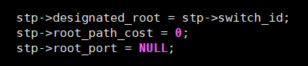
\includegraphics[width=5cm, height=2cm]{init_stp.png}
	\caption{Init switch as a root node}
	\label{init_stp}
\end{figure}

\begin{figure}[ht]
	\centering
	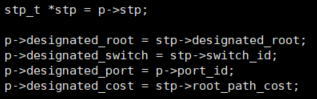
\includegraphics[width=6cm, height=2.5cm]{init_port.png}
	\caption{Init ports as DP}
	\label{init_port}
\end{figure}

Besides DPs, there're root ports (RPs) and alternative ports (APs). 
Only DPs can send config packets through their physical links.

There're three situations where config sending will be triggered.

\begin{itemize}[topsep=0pt, itemsep=0pt, parsep=0pt]
\item[(1)] For root nodes, they send config via all DPs every two seconds 
named hello time. 
\item[(2)] For all nodes, if some port receives a config with higher priority and 
updates its status, it must broadcast the new config via all the DPs.
\item[(3)] For all nodes, if some port receives a config with lower priority and the 
port is a DP, then it only need to send its config through that port.
\end{itemize}

Figure \ref{hello_timer} and Figure \ref{hello_timer_handler} are the initialization of the timer and its handler for the first situation.

\begin{figure}[ht]
	\centering
	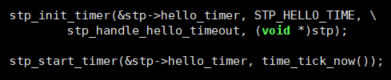
\includegraphics[width=8cm, height=2.5cm]{hello_timer.png}
	\caption{Init hello timer}
	\label{hello_timer}
\end{figure}

\begin{figure}[ht]
	\centering
	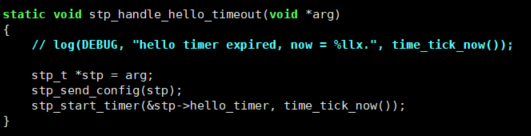
\includegraphics[width=8cm, height=2.5cm]{hello_timer_handler.png}
	\caption{Hello timer handler}
	\label{hello_timer_handler}
\end{figure}

The last two situations are resolved in the function stp\_handle\_config\_packet() in Figure\ref{stp_handle_config_packet}.

\begin{figure}[ht]
	\centering
	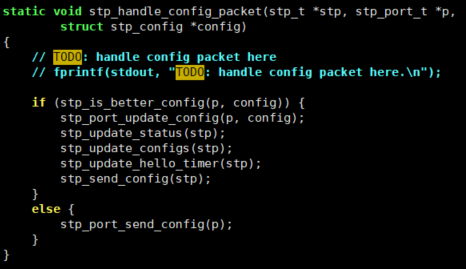
\includegraphics[width=10cm, height=4cm]{stp_handle_config_packet.png}
	\caption{STP handle received config}
	\label{stp_handle_config_packet}
\end{figure}

Note that we don't judge if the port is a DP while receiving a lower priority config.
Actually if a port is a RP or a AP, it's impossible to receive a lower priority config.
More specifically, the priority of the received config is either identical or higher
than its own config.

\section{IMPLEMENTATION}

Since the 1st or the 3rd situations is easy to fix, where we only need to send the config of the node via all DPs or a single specific DP.

They're just some portions of the entire process in the 2nd situation, so we take the 2nd situation as an example to show our STP handle procedure.

\subsection{PRIORITY JUDGEMENT}

As shown in Figure \ref{compare_priority}, once we receive a config packet, we must compare its priority with that of the node itself.

These attributes are compared one by one, which are the root id, the root path cost, the switch id and the port id.

\begin{figure}
	\centering
	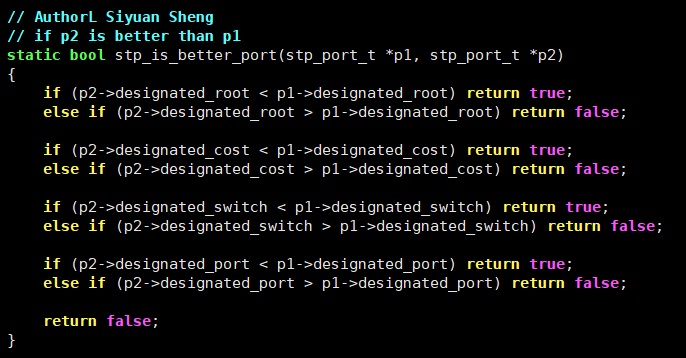
\includegraphics[width=10cm, height=4cm]{compare_priority.png}
	\caption{Compare priority}
	\label{compare_priority}
\end{figure}

\subsection{PORT CONFIG UPDATE}

Since we take the 2nd situation as our example, the priority of incoming ocnfig is higher than the original one of the node itself. So we should udpate the config of the specific port which received the better config.

As Figure \ref{port_update_config} shows, we copy the information of incoming config into that port directly.
According to Figure \ref{is_designated}, we can distinguish whether a port is a DP through its switch id and port id. So after updating the ports' config, its switch id and port id changes, thus it has been converted into a AP automatically.

\begin{figure}
	\centering
	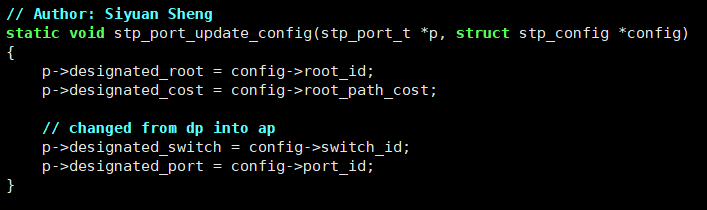
\includegraphics[width=10cm, height=4cm]{port_update_config.png}
	\caption{Update port config}
	\label{port_update_config}
\end{figure}

\begin{figure}
	\centering
	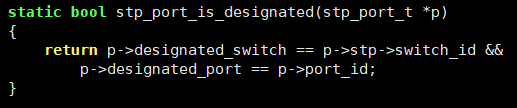
\includegraphics[width=8cm, height=2.5cm]{is_designated.png}
	\caption{Judge DP}
	\label{is_designated}
\end{figure}

\subsection{NODE STATUS UPDATE}

After updating the ports' config, we need to update the status of the entire node as Figure \ref{update_status}.

First we try to select a port with the highest priority among all APs as the root port (RP), which indicates the root path of the node in the spanning tree.

Then if RP exists, we update the nodes' config based on the RPs' config. Otherwise if we don't find RP which means the node is a root switch, we should update the nodes' config as a root node, just like what we do in the init phase.

\begin{figure}
	\centering
	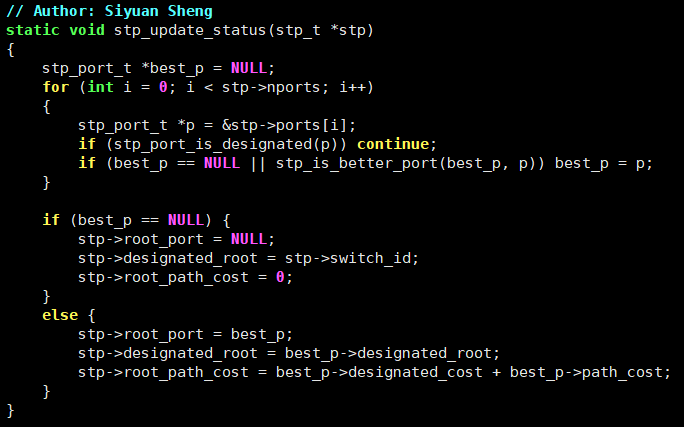
\includegraphics[width=10cm, height=4cm]{update_status.png}
	\caption{Update node status}
	\label{update_status}
\end{figure}

\subsection{OTHER PORTS CONFIG UPDATE}

We have udpated the specific ports' config which receives the packet with the incoming config.
Now we must udpate configs of all the other ports including both APs and DPs.

As Figure \ref{update_configs}, we traverse all the APs one by one to see if we need to convert anyone into DP. Anyway, we choose some APs and reset their switch ids and port ids as DPs. The details have been demonstrated in the codes of Figure \ref{update_configs}, here let's just skip it.

Finally, we update the configs of all DPs including the new converted ones.

\begin{figure}
	\centering
	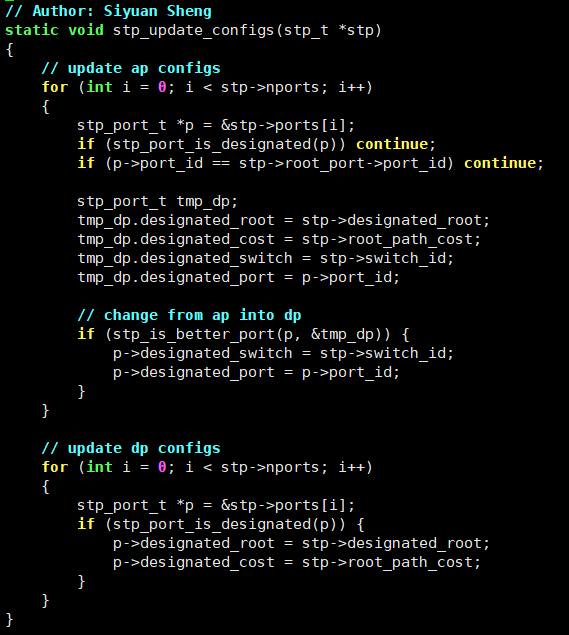
\includegraphics[width=7cm, height=9cm]{update_configs.png}
	\caption{Update other ports' configs}
	\label{update_configs}
\end{figure}

\subsection{OTHER PORTS CONFIG UPDATE}

This step is quite simple in Figure \ref{update_hello_timer}.
We just reset the hello timer or stop it according to whether the node is still a root switch or not.

\begin{figure}
	\centering
	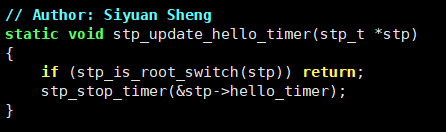
\includegraphics[width=6cm, height=2.5cm]{update_hello_timer.png}
	\caption{Update hello timer}
	\label{update_hello_timer}
\end{figure}

\subsection{SEND CONFIG}

At last, we need to send configs through all the DPs of the node as Figure \ref{send_config}. The 1st situation where the hello timer is trigger, just need to call this step directly.

In the function stp\_send\_config(), it calls stp\_port\_send\_config() for each DP.

\begin{figure}
	\centering
	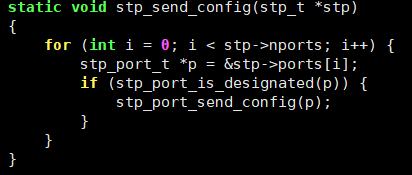
\includegraphics[width=6cm, height=2.5cm]{send_config.png}
	\caption{Send config}
	\label{send_config}
\end{figure}

In Figure \ref{port_send_config}, we package the config of the port into a STP packet whose format is ether\_header + llc\_header + stp\_config (stp\_header + other fields).

By the way, the ether\_header is actually a redundant structure since we get the same information from the frame header. And the llc\_header and some fields of stp\_config aren't used in our simplified STP implementation.

\begin{figure}
	\centering
	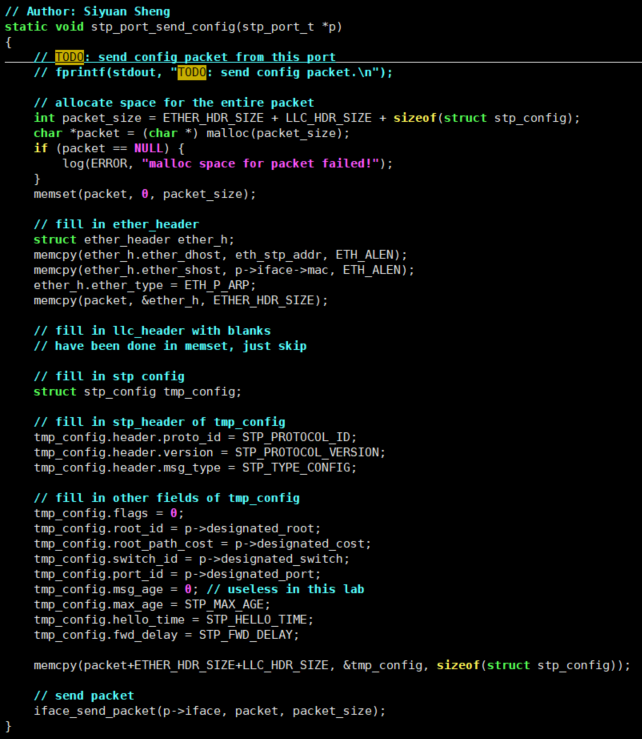
\includegraphics[width=10cm, height=12cm]{port_send_config.png}
	\caption{Port send config}
	\label{port_send_config}
\end{figure}

\section{EXPERIMENTS}

\subsection{FOUR-NODE TOPOLOGY}

As in Figure \ref{four_node_topo}, it's our four-node topology. 
Figure \ref{four_our_own} shows our own output of this topology.
Figure \ref{four_reference} shows reference output of this topology.

If you want to take a look at these outputs in detail, just open the directory under my project ./outputs/four.txt and ./outputs/four-reference.txt.

\begin{figure}
	\centering
	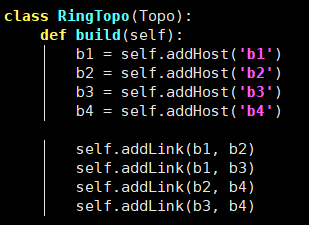
\includegraphics[width=7cm, height=5cm]{four_node_topo.png}
	\caption{Four node topology}
	\label{four_node_topo}
\end{figure}

\subsection{SEVEN-NODE TOPOLOGY}

As in Figure \ref{seven_node_topo}, it's our seven-node topology. 
We won't show the figures of our own output and the reference output because of the space limit.

If you want to take a look at these outputs in detail, just open the directory under my project ./outputs/seven.txt and ./outputs/seven-reference.txt.

\begin{figure}
	\centering
	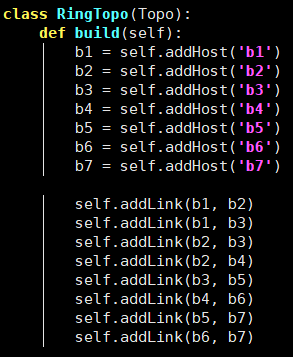
\includegraphics[width=7cm, height=7cm]{seven_node_topo.png}
	\caption{Seven node topology}
	\label{seven_node_topo}
\end{figure}

\begin{figure}
	\centering
	\subfigure[Our own output]
	{
		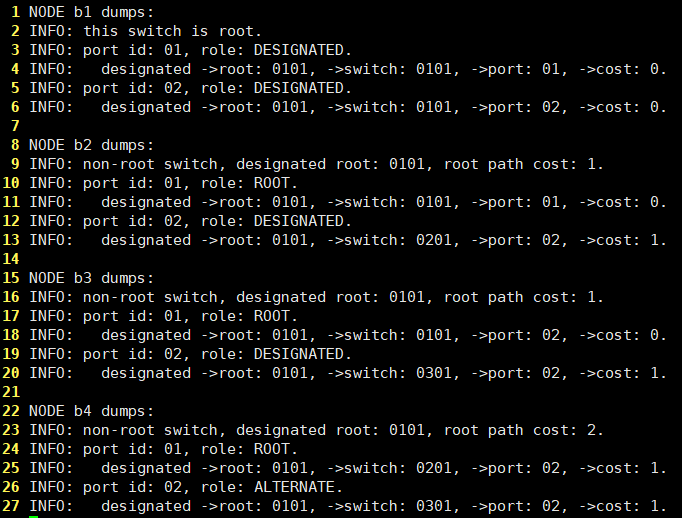
\includegraphics[width=5cm, height=9cm]{four_our_own.png}
		\label{four_our_own}
	}
	\subfigure[Reference output]
	{
		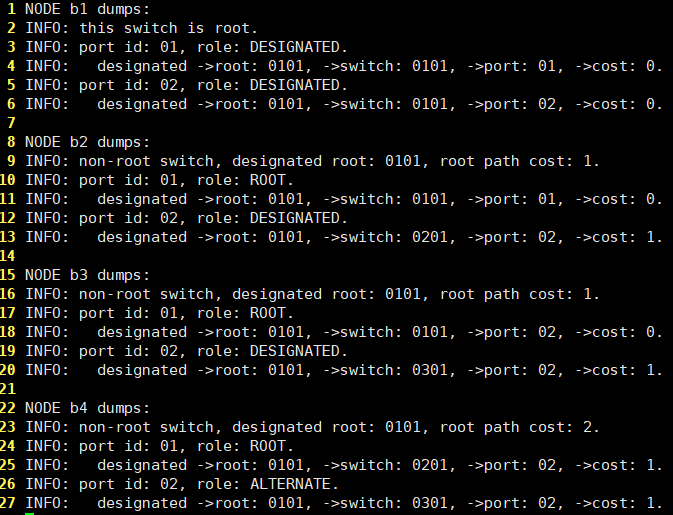
\includegraphics[width=5cm, height=9cm]{four_reference.png}
		\label{four_reference}
	}
	\caption{Compare outputs of four-node topology}
	\label{four_outputs}
\end{figure}

\end{document}